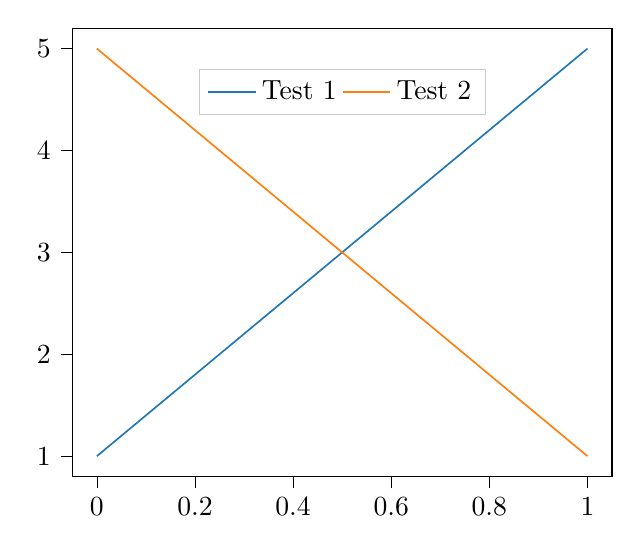
\begin{tikzpicture}

\definecolor{darkgray176}{RGB}{176,176,176}
\definecolor{darkorange25512714}{RGB}{255,127,14}
\definecolor{lightgray204}{RGB}{204,204,204}
\definecolor{steelblue31119180}{RGB}{31,119,180}

\begin{axis}[
legend cell align={left},
legend columns=2,
legend style={
  fill opacity=0.8,
  draw opacity=1,
  text opacity=1,
  at={(0.5,0.91)},
  anchor=north,
  draw=lightgray204
},
tick align=outside,
tick pos=left,
x grid style={darkgray176},
xmin=-0.05, xmax=1.05,
xtick style={color=black},
y grid style={darkgray176},
ymin=0.8, ymax=5.2,
ytick style={color=black}
]
\addplot [semithick, steelblue31119180]
table {%
0 1
1 5
};
\addlegendentry{Test 1}
\addplot [semithick, darkorange25512714]
table {%
0 5
1 1
};
\addlegendentry{Test 2}
\end{axis}

\end{tikzpicture}
